\documentclass[11pt]{article}

% Paquetes de texto:
\usepackage[english]{babel}
\usepackage[utf8]{inputenc}
% Paquetes para incluir graficos:
\usepackage{graphics}
\usepackage{graphicx}
\usepackage{epstopdf}
% Tratamiento de graficos
\usepackage{picture}
% Colores
\usepackage[usenames]{color}
% Texto preformateado
\usepackage{verbatim}
\usepackage{listings}
% Hipervinculos (indice y URLs)
\usepackage{hyperref}
% Matematicas
\usepackage{amsfonts}
\usepackage{amsmath}
\usepackage{amsthm}
\usepackage{amssymb}
\usepackage{anysize}
\usepackage[hypcap]{caption}
\usepackage{geometry}
\usepackage[final]{pdfpages}

\newcommand{\HRule}{\rule{\linewidth}{0.5mm}}

%%PER EL CODI EN C%%%
\usepackage{listings}
\lstset{ %
language=C++,                % choose the language of the code
basicstyle=\footnotesize,       % the size of the fonts that are used for the code
numbers=left,                   % where to put the line-numbers
numberstyle=\footnotesize,      % the size of the fonts that are used for the line-numbers
stepnumber=1,                   % the step between two line-numbers. If it is 1 each line will be numbered
numbersep=5pt,                  % how far the line-numbers are from the code
backgroundcolor=\color{white},  % choose the background color. You must add \usepackage{color}
showspaces=false,               % show spaces adding particular underscores
showstringspaces=false,         % underline spaces within strings
showtabs=false,                 % show tabs within strings adding particular underscores
frame=single,           % adds a frame around the code
tabsize=2,          % sets default tabsize to 2 spaces
captionpos=b,           % sets the caption-position to bottom
breaklines=true,        % sets automatic line breaking
breakatwhitespace=false,    % sets if automatic breaks should only happen at whitespace
escapeinside={\%*}{*)}          % if you want to add a comment within your code
}



%\marginsize{3 cm}{2 cm}{2 cm}{2.5 cm}

%\title{\textbf{Project Handbook for Development Projects}}
%\author{Carolina Millet \\ Xavier Bush}
%\date{Spring 2015}		% Comentar para que aparezca la fecha de hoy
\newgeometry{
    top=35mm,
    bottom=30mm,
    outer=30mm,
    inner=30mm,
}

\begin{document}


\begin{titlepage}
\begin{center}


\textsc{\LARGE Kungliga Tekniska Högskolan}\\[1.5cm]

\textsc{\Large ~}\\[-0.5cm]


\HRule
{ \huge \bfseries \textbf{Project Plan} \\ Noise and echo cancellation in a teleconference \\ Project in Wireless Communication \\[0.4cm] }

\HRule \\[1.1cm]

% Author and supervisor
\begin{minipage}{0.4\textwidth}
\begin{flushleft}
\emph{Authors:}\\
Animesh Das \\ Jonas Sedin \\ Mohammad Abdulla \\ Thomas Gaudy \\ Xavier Bush
\end{flushleft}
\end{minipage}
~
\begin{minipage}{0.4\textwidth}
\begin{flushright}
\emph{Advisor:}\\
Per Zetterberg
\end{flushright}
\end{minipage}

\vfill

% Bottom of the page
{\large Spring 2015} \\[1cm]
\end{center}



\end{titlepage}
\restoregeometry   



\pagebreak\tableofcontents
\pagebreak
\section{Introduction}

This is the Project Plan of the Project in Wireless Communication \textit{ Noise and echo cancellation in a teleconference}. As a project plan, this is also the contract between the team members and the supervisor of the Project, Per Zetterberg, that contains the goals, the organisation, the resource plan, the risk analysis, the documents rules and the project model that the project follows.

\section{Background}

This project intends to be the first real project where to apply the theoretical knowledge acquired in the KTH's Master performed by the team members. Moreover, all the experience to gain during the project such as team work, project management, code programming and application of theory into practice were taken into account to choose the project, and all of these competences will be used when performing our Master Thesis next year.

In the following sections, the Project Plan will be developed in detail with the aim to follow it as good as possible and to show it to the project supervisor (sponsor).


\section{Specification of the project}

The aim of the project, as the title of itself says, is to program a noise and echo cancellation algorithm in a teleconference in real time. The very first scenario (Figure \ref{scenario}) considers that only one of the users is speaking in an echo and noisy environment. Further in the project, if the first scenario is successfully solved, a second scenario will be approached: both users might be in a echo and noisy environment.

		\begin{figure}[h]
		\centering
		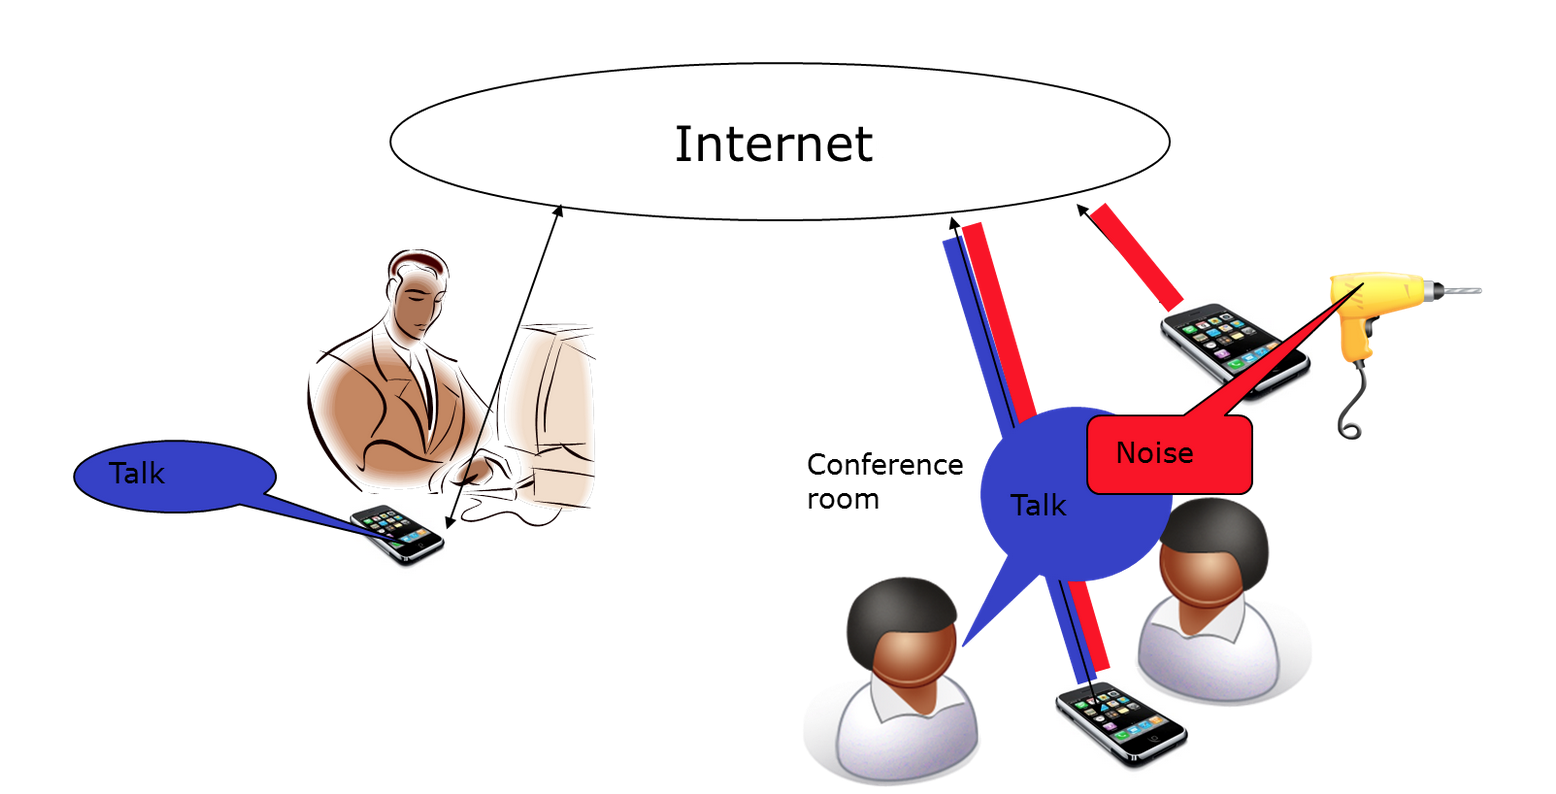
\includegraphics[width=10cm]{scenario}
		\caption{Illustration of teleconference with noise (interference) cancellation}
		\label{scenario}
		\end{figure}

\section{Sketch of solution}


With a needed background in adaptive signal processing and programming, mostly in MATLAB and Android, the goal is to cancel the noise and the echo generated in the user's environment during a teleconference (Figure \ref{scenario}). To do so, the group will use mostly the content of the course \textit{Adaptive Signal Processing (EQ2400)} and therefore mode and test the system in a theoretical way. The test of the algorithms will be done by MATLAB and the implementation in real time will be coded with Android in the Eclipse environment. As there are 5 members in the team and different areas where to work, everyone has been allocated in these areas with certain responsabilities (see \textit{Organisation}) and will report properly the progress of the project.
		
The first approach to solve the problem will be by using Adaptive Signal Processing techniques. In order to work the project, the team has been provided 5 cellphones to work with:

\begin{itemize}
\item 2 phones for the users (1 phone per user)
\item 1 phone as a server
\item 1 phone to record the noise
\end{itemize}

With the information of the recorded noise, adaptive filtering techniques such as LMS will be used as noise cancellation tools. In terms of echo cancellation, the team still have to look deeper into it but the first approach will be LMS as well. Anyway, there are different possibilities to analyze before starting the MATLAB program because the model can be slightly modified:

\begin{itemize}
\item Order of the cancellation: first echo cancellation and second the noise cancellation or vice versa
\item The cancellation should be done in the server or in the receiver. Seems more reasonable the receiver option but all possibilities will be taken into account
\end{itemize}


Finally the first model that will be used to treat the noise is show in the Figure \ref{model}. On the other hand, the echo cancellation will follow a similar model but the CIOs need to study deeper the final model.

		\begin{figure}[h]
		\centering
		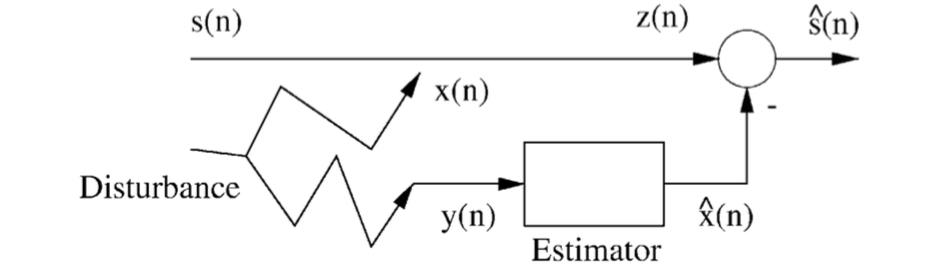
\includegraphics[width=10cm]{model}
		\caption{Model of noise cancellation}
		\label{model}
		\end{figure}

\section{Goals}

The goals of the team can be divided in two academic goals (business goals) and project goals. The academic goal is to achieve the best result within the time constrain given by the course (8 weeks). Consequently, the minimum score required will be a \textbf{B} being \textbf{A} the desired mark. In terms of project goals, as engineers the project should fulfill the expectation of noise and echo cancellation with the minimum possible delay, in order to have a real time application.

Due to the complexity of the project, the budget (hours invested by the team members) will not be a constrain (in comparison with the time and the quality). Even though, every member of the team has other courses or seminars to attend, which will turn into risk factors that may affect during the performance of the project (see \textit{Risk Analysis}). According to the previous information, the Figure \ref{3_const} shows the triple constraint of the project.


		\begin{figure}[h]
		\centering
		\includegraphics[width=10cm]{tripleconstrain}
		\caption{Triple constrain of the project}
		\label{3_const}
		\end{figure}

\section{Organisation}

The organisation is fully made up by electrical engineering students. Each of the team members perform a different role and most of the members work in two different areas. The reason of working in different areas make easier the knowledge transfer in this areas, fact that will make the project run faster. The members, their roles and contact information are specified below:

\begin{itemize}

\item Animesh Das
	\begin{itemize}
	\item Role: Theory Group \& Management Group
	\item e-mail:animeshu1989@gmail.com (animeshd@kth.se)
	\item Telephone: +46 737155575
	\end{itemize}
	
\item Jonas Sedin
	\begin{itemize}
	\item Role: Theory Group \& Android Group
	\item e-mail: sedinjo@gmail.com (jonassed@kth.se)
	\item Telephone: +46 704252951
	\end{itemize}
	
\item Mohammad Abdulla
	\begin{itemize}
	\item Role: Android Group
	\item e-mail: hamodiilatch@gmail.com (mabdulla@kth.se)
	\item Telephone: 
	\end{itemize}
	
\item Thomas Gaudy
	\begin{itemize}
	\item Role: Android Group
	\item e-mail: gaudy.thomas@gmail.com (gaudy@kth.se)
	\item Telephone: +46 760936034
	\end{itemize}
	
\item Xavier Bush
	\begin{itemize}
	\item Role: Theory Group \& Management Group
	\item e-mail: xavier.bush@gmail.com (xbush@kth.se)
	\item Telephone: +46 764141834
	\end{itemize}
	
	
\end{itemize}

The sponsor members as Project Examiner/Supervisor and Project Support are:

\begin{itemize}
\item Per Zetterberg
	\begin{itemize}
	\item Role: Project Examiner
	\item e-mail: perz@ee.kth.se
	\item Telephone: +46 8 790 77 85
	\end{itemize}
	
\item Hadi Ghauch
	\begin{itemize}
	\item Role: Group Assistant
	\item e-mail: ghauch@kth.se
	\end{itemize}
	
\item Martin Ohlsson
	\begin{itemize}
	\item Role: Android Guru
	\item e-mail: martinoh@kth.se
	\item Telephone: +46 87907818
	\end{itemize}
\end{itemize}

\section{Tasks \& Time and Resource Allocation Plan}

\subsection*{Tasks}
As it has previously said, the tasks of the project have been distributed among the team members depending on the areas of work. All the tasks with its classification, type of task, date to be ready and responsible, have been distributed as shown in the \textit{Annex 1}. Due to the \textit{Mid-term evaluation} the Android tasks have been distributed among the team's programmers depending on the comlexity of the task and the ammount of phones involved. Eventually, tasks 1, 2, 3 and 4 will be done individually and tasks 5, 6 and 7 will be done by groups.\\

On behalf of the Theory team, there are three phases involved: noise cancellation, echo cancellation and the merge of these two procedures (with code optimizing and transfer from MATLAB to Android). All the details in the \textit{Annex 1}.\\

Finally, the Management area will take care about the Project Plan, all the Status Reports of the project and the Final Report. All the detailes, again, in the \textit{Annex 1}.

\subsection*{Time and Resource Allocation Plan (TRAP)}
The measurable resources of the team is the amount of hours to dedicate to the project, and it has been planned as a \textit{Time and Resource Allocation Plan}. Considering this, each of the members will work, a priori, 4 hours per day and 4 days per week, with some exceptions in the weeks with more work. After a first test in certain assignments it is a reasonable amount of hours with a total close to 190 hours in the 8 weeks of the course.

In order to plan the hours to dedicate and make a right follow up of them, it has been done a document named \textit{TimeAndResourcePlan.xls} this document is attached in this Project Plan as the \textit{Annex 2} As a clarification, the hours that stated in the Time and Resourse Allocation Plan are effective hours in the laboratory, the self study is not included. As it can be seen, the \textit{Outcome} row is the follow-up of the hours a posteriori, when the \textit{Plan} row is the planned hour. The goal in this section is to have the same amount of hours in both rows, meaning that that the plan has been succesfuly done.

\subsection*{Gantt Chart}
At the end of this document, and follow a similar structure of the \textit{Annex 1} this project's Gantt Chart can be found. Te total amount of weeks of the Gantt Chart is 11 where all the tasks have been allocated on behalf of the group where does everyone of them belong to. The \textit{3rd} level classification has not been allocated to a responsable or to a certain time frame because all the \textit{3rd} level tasks feedback each other and will not follow a certain order between them.

\section{Risk Analysis}

In terms of risks that may affect the project we have analyzed two types of them:

\begin{itemize}
\item Technical risks: involving all the technical risks or lack of knowledge that the team may find during the project. This risks are unmeasurable and uncertain since Android programming and real time application are new areas for the team members and problems of different nature may occur.

\item Managerial risks: all external risks that might put in difficulty the right follow up of the Project Plan. This section contains other courses, seminars, projects and language courses that the team members follow simultaneously.

\end{itemize}

In this Risk Analysis have not been taken into account personal activities or situations of the course members understanding that each member of the team should handle them so not to affect the performance of the project. For this reason, Table \ref{tablerisk} shows the risk table done following the \textit{Mini-Risk Method} (``Handbook for Small Project''), where \textbf{P}=Probability that the risk happens (from 1 to 4), \textbf{C}=consequence if the risk happens (from 1 to 4) and \textbf{R}=Risk Value (from 1 to 16).


\begin{table}[h]
\centering
\begin{tabular}{l| l| l| l| l| l}
 Nr &Risk  &P  &C  &R &Action  \\
 \hline
 1 & Do not find a good theoretical model & 1 & 4 & 4 & Read more literature\\
 2 & Do not pass the mid-term evaluation & 1 & 4 & 4 & Re-schedule the TRP\\
 3 & Problems with real time & 2 & 4 & 8 & Help and re-schedule TRP \\
\end{tabular}

\label{tablerisk}
\end{table}



\section{Documents and Rules}
This section contains the rules to follow in terms of documentation during the project, some of them will be handled by the team's Managament Group and some of them will be handled individually. The projects to be done during the project will be next:

\begin{itemize}
\item Project Plan: will be done by Xavier at the beginning of the project. The hand in it in will be done by posting it in the project's KTH social group.

\item Reflective diary: this document will be done individually. Will be handled by e-mail to Per Zetterberg in pdf or .doc file before the deadline indicated by the schedule. Should include all what each team member has done in a schematic way with all the documentation needed to suport the lyrics.

\item Progress Report: will be done by the Animesh and handed in before the deadline of the schedule. As the Project Plan, it will be posted in the porject's KTH social group.  All the information will be provided by the team members to Xavier so to elaborate this document.

\item Final Report: will be done by the Xavier with all the information provided by the Theory Group and Android Group before the deadline of the course.
\end{itemize}


The backup of the information will be don daily using next sources:

\begin{itemize}
\item Github: the group has a shared github server. All the progress will be uploaded at the end of the day
\item Hard Disk: Every member of the team will have a daily backup in his own machine
\end{itemize}

With this backup procedure there will be at least 3 copies a day of the project.

\section{Project Model}

The project model will follow the general Project Flow (Ref. Handbook for Small Projects, Joakim Lilliesköld). In the Annex 1 can be found a Schedule with all the deadlines and important dates during the project and to which phase it refers to and so who is responsible of each task. The project is divided into next phases:

\begin{itemize}
\item Pre-study: already done before taking the course
\item Start: Will finish when the Project Plan will be finished and approved
\item Execution: Will last from the 1st of April until the 31st of May
\item Closing: Will finish with the last \textit{Reflective Diary}
\end{itemize}

Milestones and Tollgates will be used to organise the project. On the one hand, Milestones will be considered as checkpoints defined by the team members to check the status of the project before a deadline. On the other hand, Tollgates will be the checkpoints of approval from the sponsor (course examiner) after a certain deadline. So as the project is short (8 weeks) and the amount of taks is considerably high it has been assigned only 1 Milestone before every deadline plus a weekly meeting to check the status of the project. Due to the small size of the team, the meeting will not be always scheduled at the same day, but preferably at the end of the week.

\section{Bibliography}


\begin{itemize}
\item Eriksson, M \& Lilliesköld, J. (2010) \textit{``Handbook for Small Projects''}. Stockholm: Liber.
\item Slides of Lectures from the course Adaptive Signal Processing (EQ2400)
\item Slides of Lectures of the course Project in Wireless Communication (EQ2440)
\end{itemize}

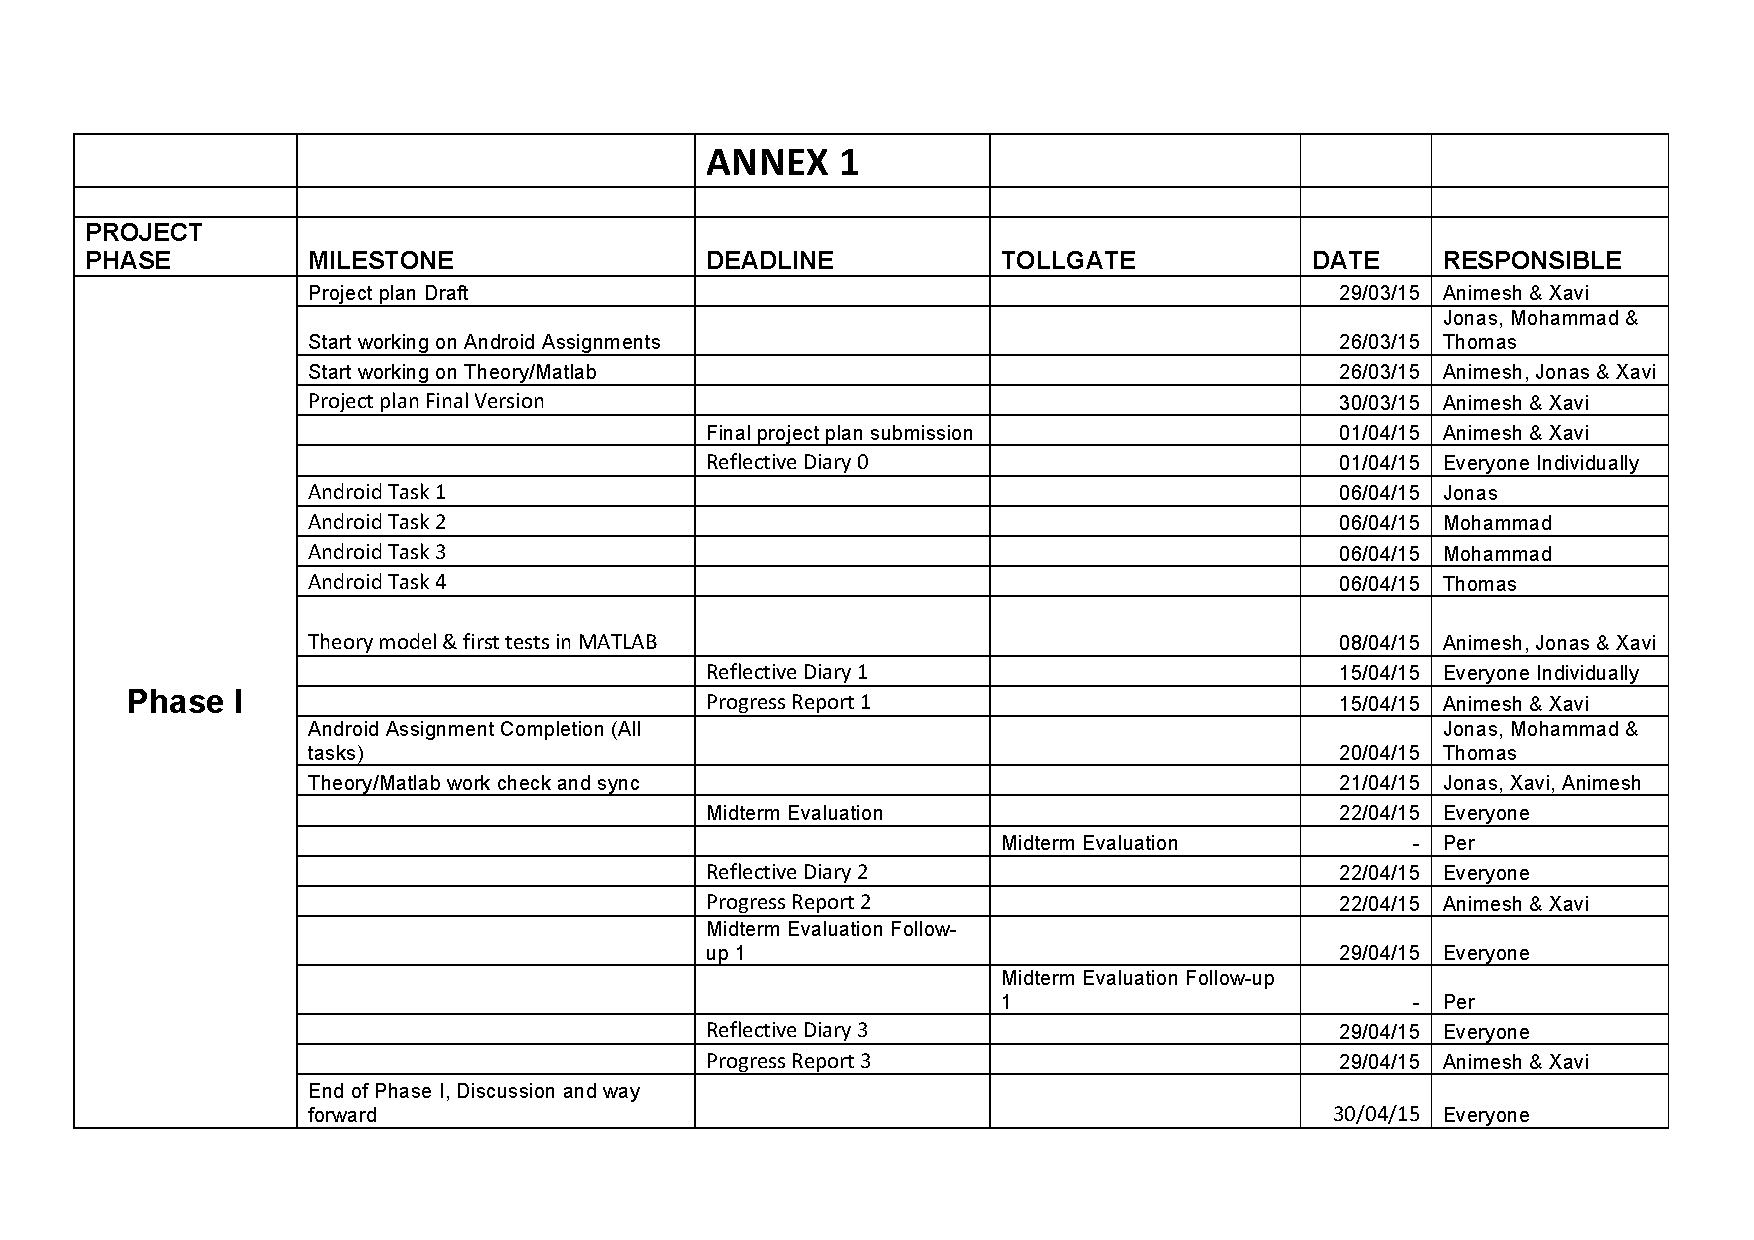
\includepdf[pages={1}]{tasks_phase1}
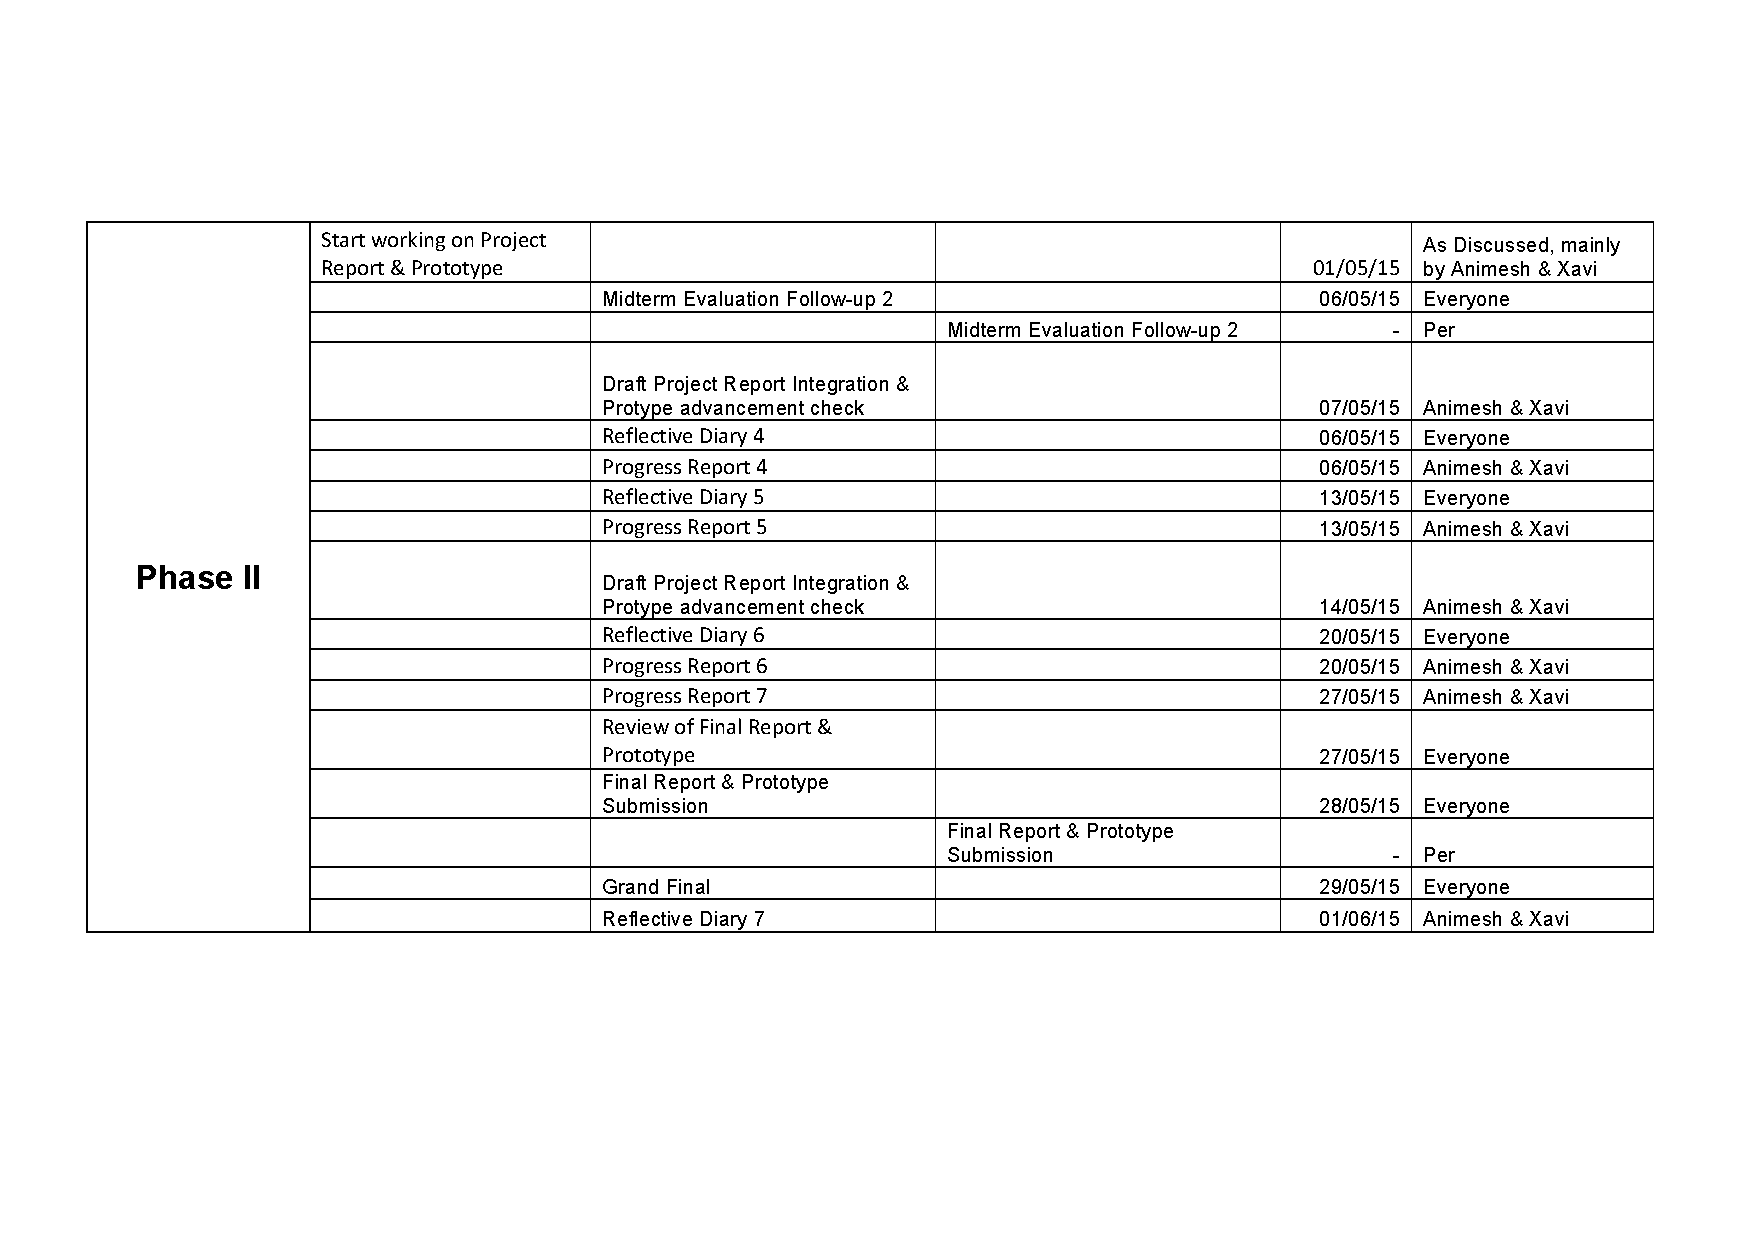
\includepdf[pages={1}]{tasks_phase2}
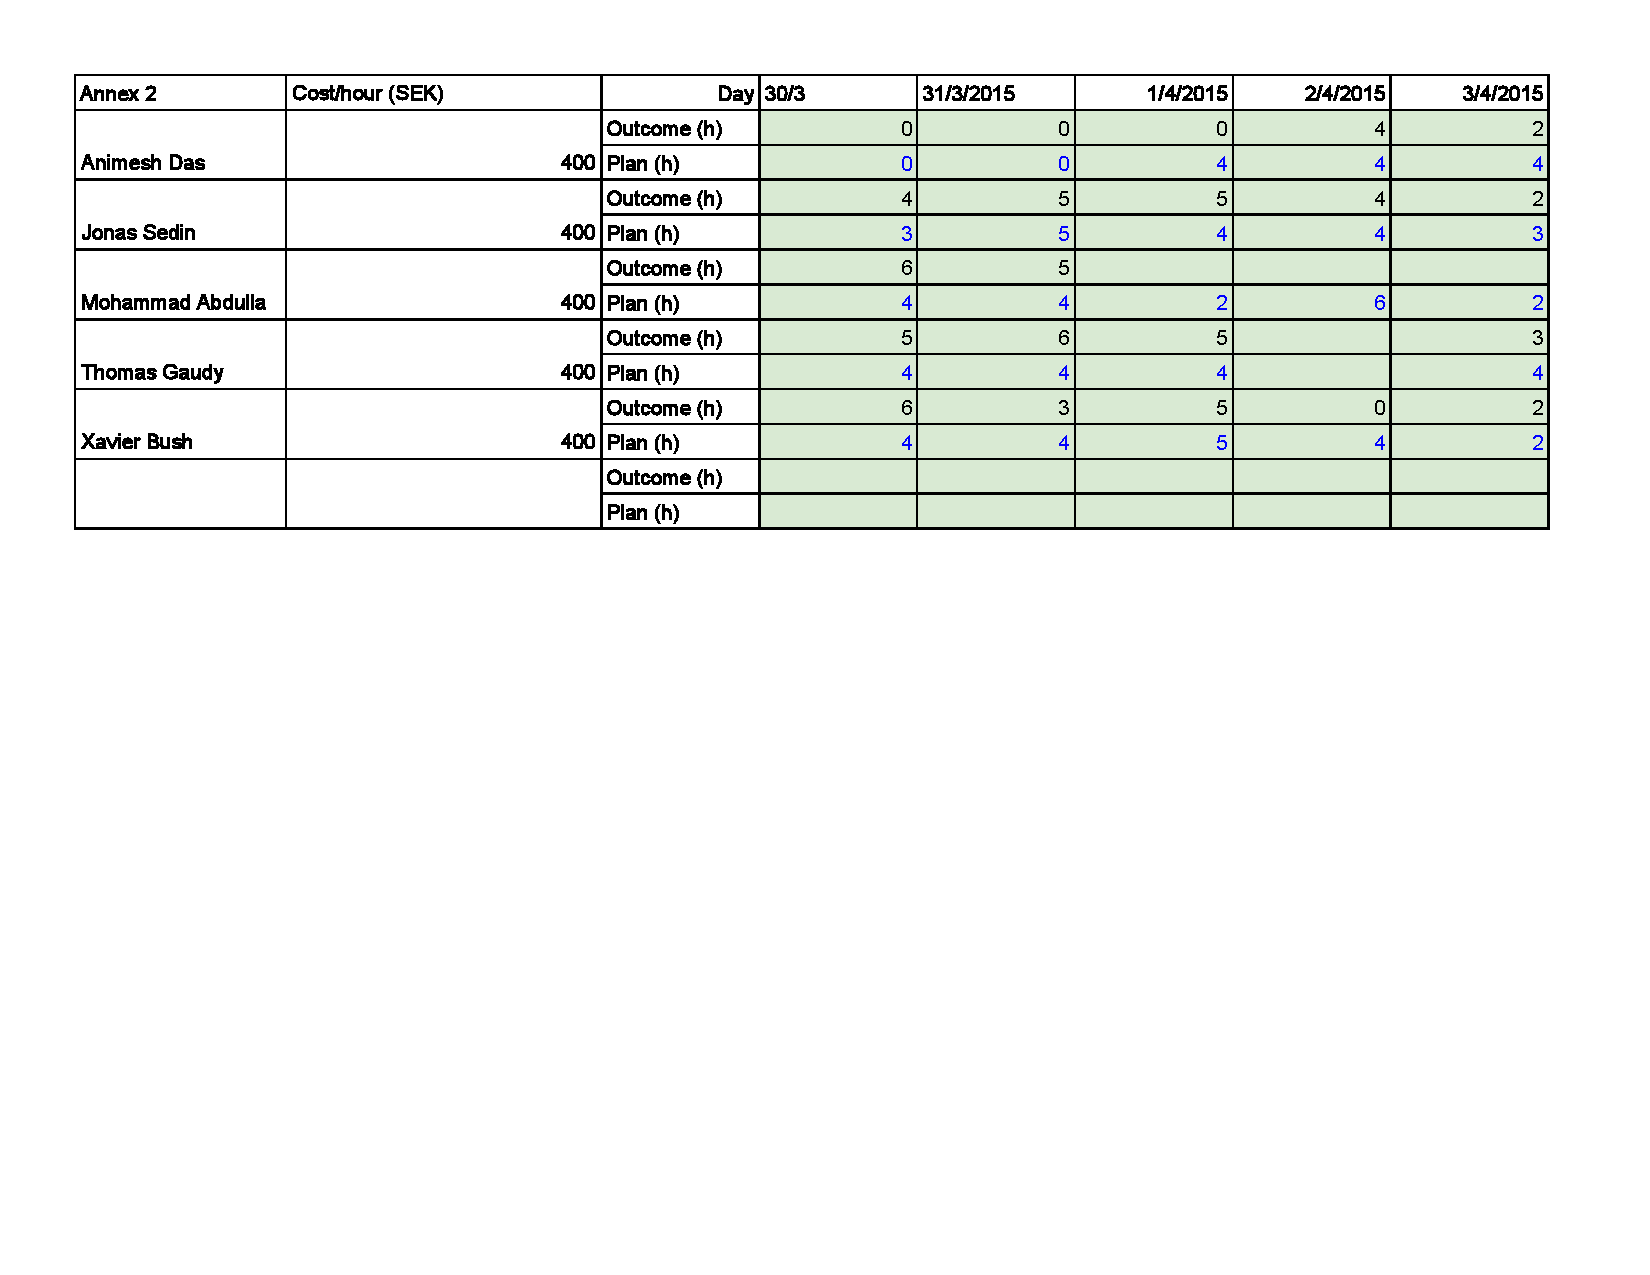
\includepdf[pages=-]{TimeResourcePlan}
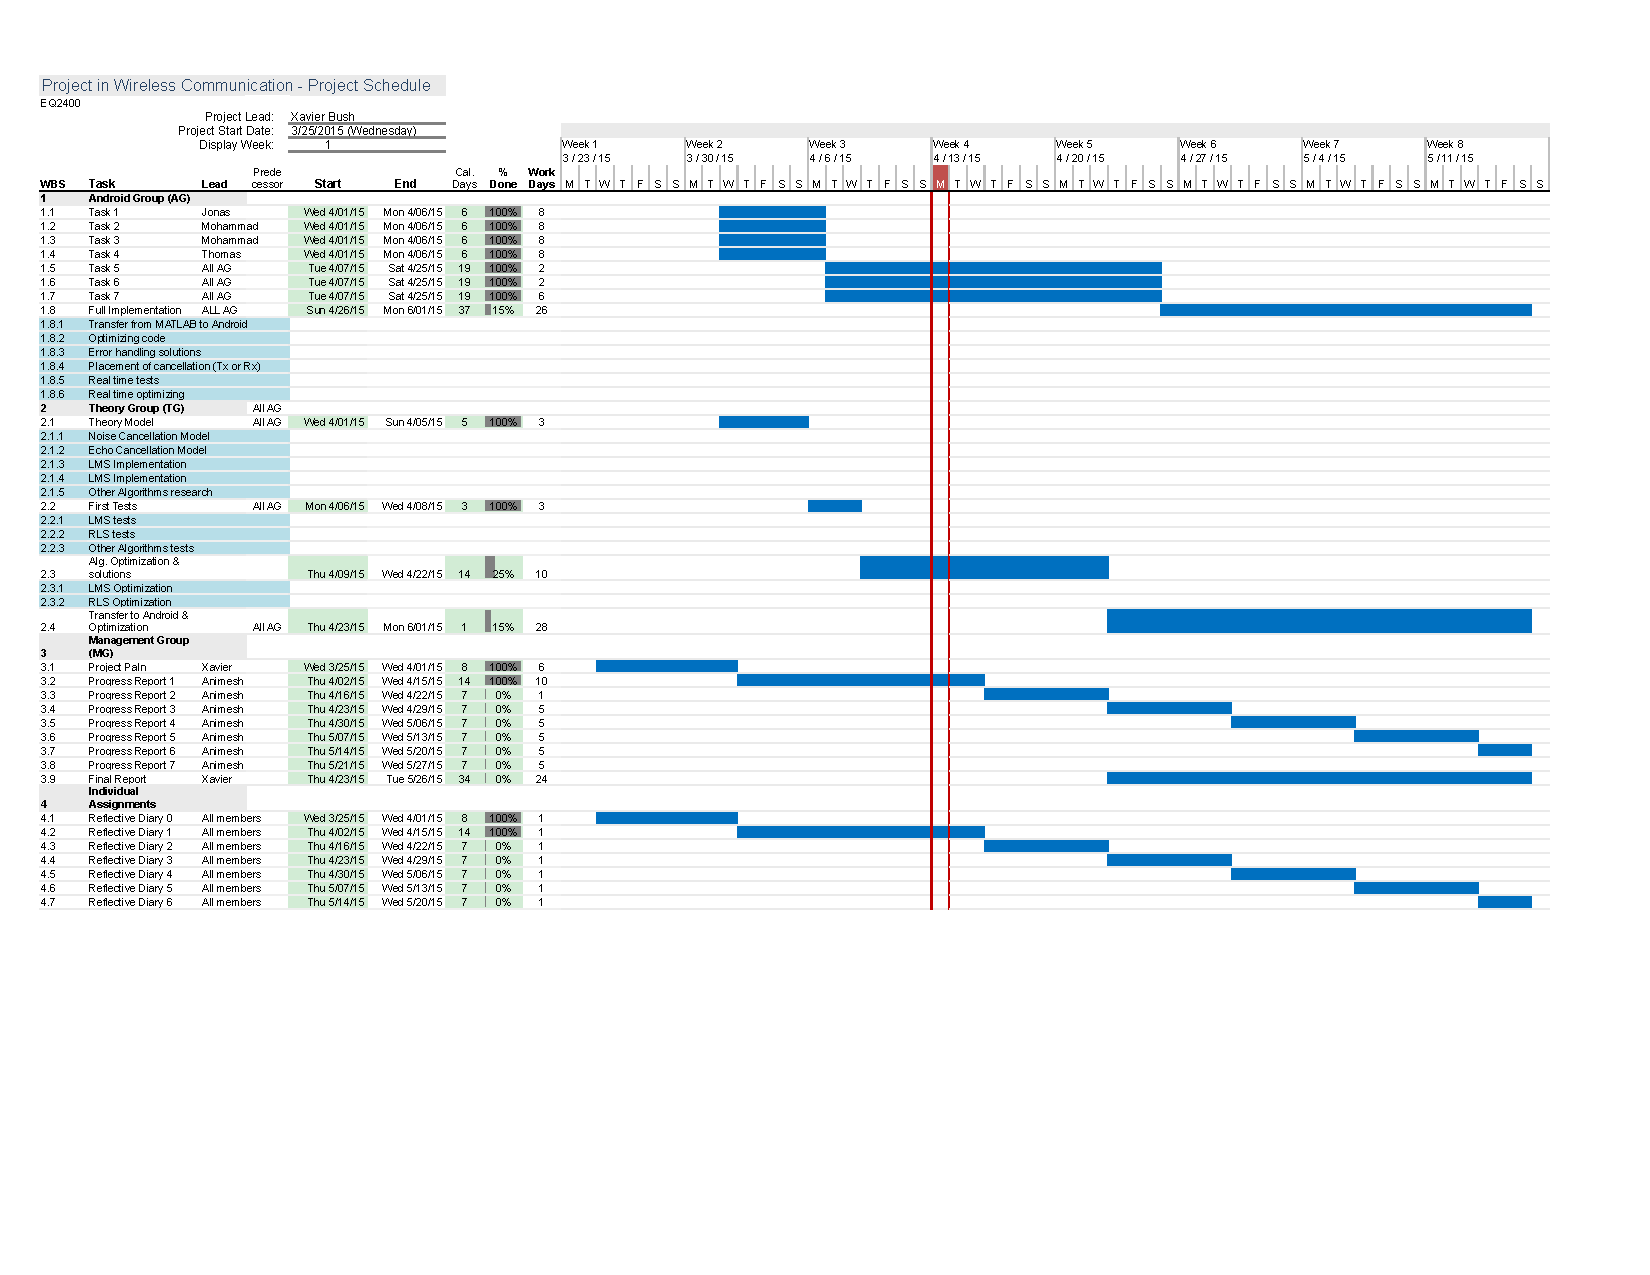
\includepdf[pages={1}]{gantcharweek1-8}
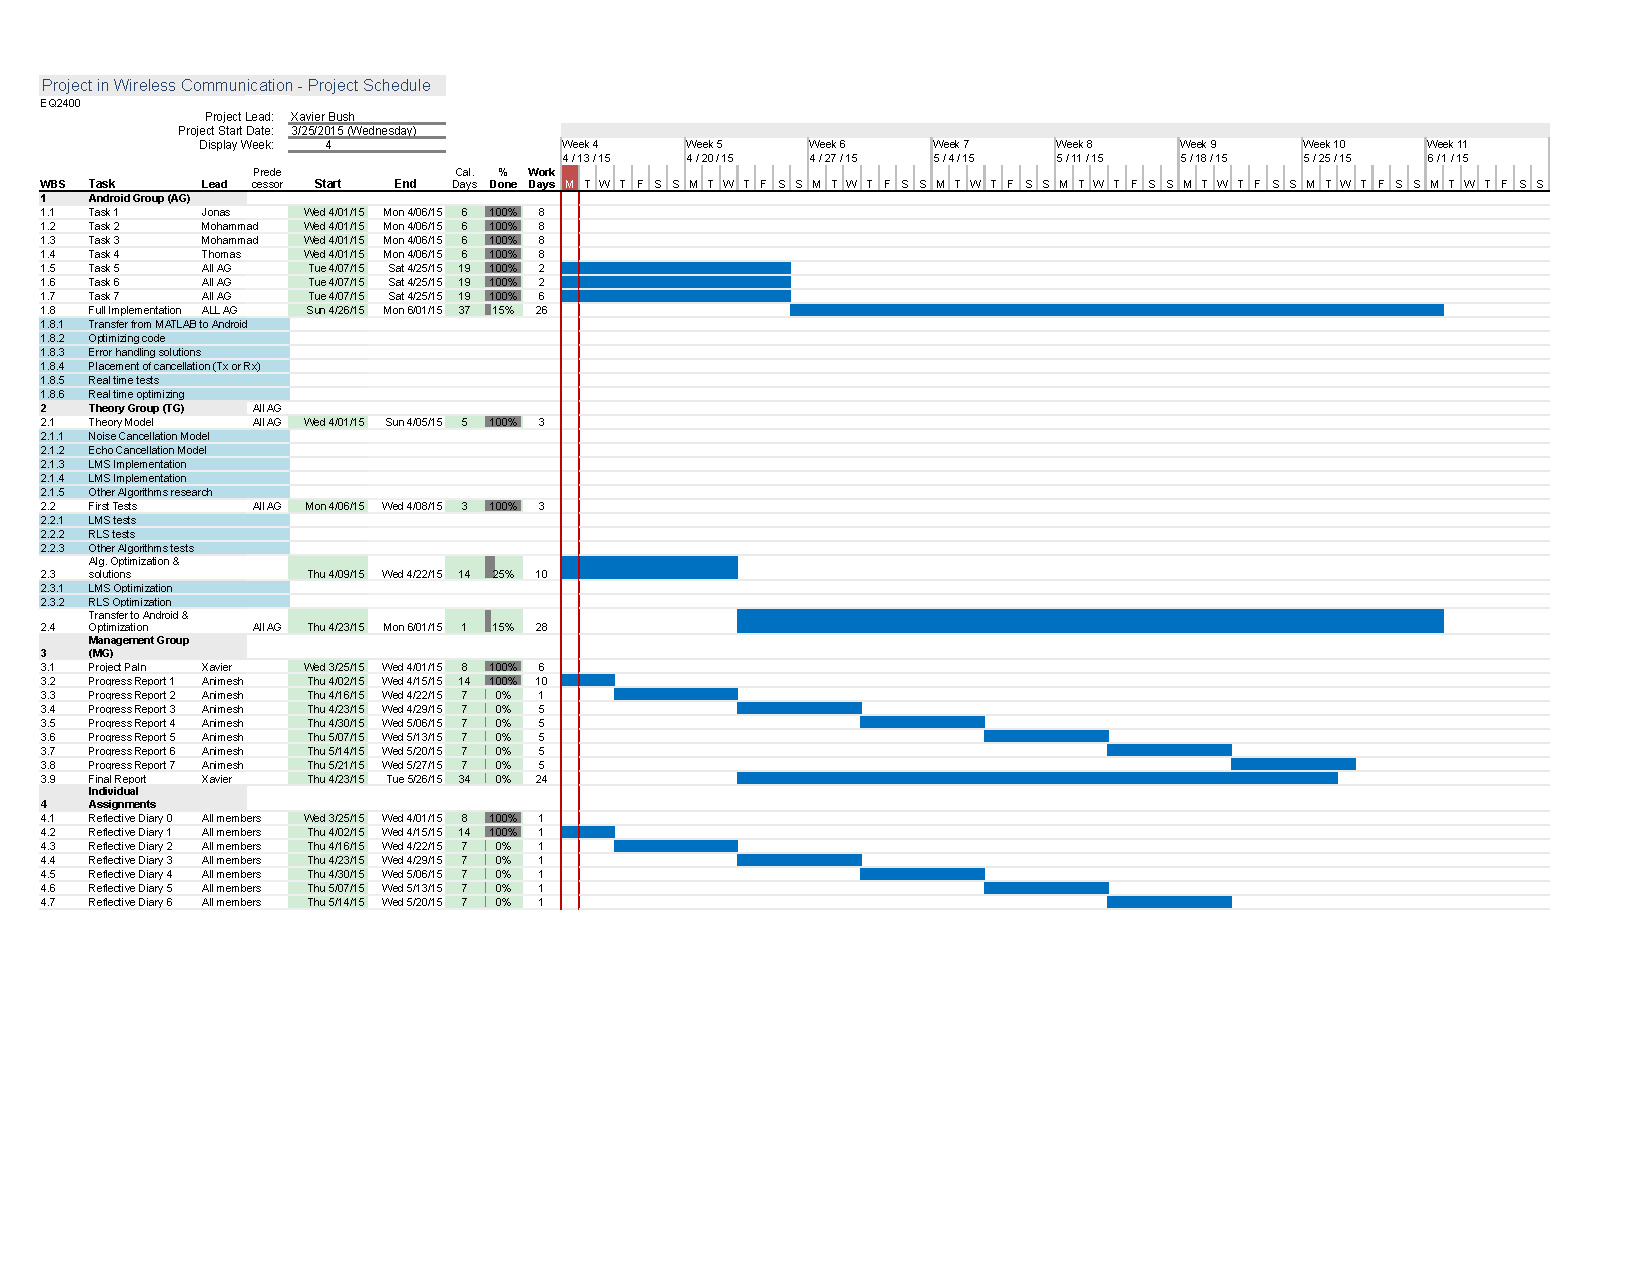
\includepdf[pages={1}]{gantcharweek8-11}

\end{document}  